\section{Introduction}

A maximum independent set (MIS) selects assignments no two of which are incompatible, and a delivered set can be checked edge by edge against the input. That makes MIS a clean testbed: the answer names the vertices, so a caller can use it the moment it arrives. A solver that has found a large independent set may still be useless to a caller that needs the answer now. On 1,000 large RB graphs under a 50~ms budget, our solver holds a feasible set on the host in all 3,000 runs, yet 475 calls still return after that deadline. Neural MIS solvers are usually scored on objective value after a fixed number of steps or a fixed wall-clock slice, and neither number says when a feasible set became readable. We take delivery as the unit of measurement. Each candidate set is copied to a host archive and timestamped; the score at deadline \(B\) is the largest set in the archive at \(B\); the solver's return time is recorded separately. The archive stores vertices, so every scored set is re-checked against the input edges after timing.

This rule exposes a choice that objective-at-return hides: what the network should do with its budget. We study SPRINT, a solver family with two routes to an answer. SPRINT-S, the speculative route, uses a particle policy built on regularized Langevin dynamics \citep{feng2025regularized}, which updates many binary states in parallel. Those states may contain adjacent vertices, so each publication must first be decoded into an independent set, and every decode competes with search. SPRINT-C, the constructive route, instead builds a maximal independent set, publishes it, and calls the network once to rank vertices for exchanges and branch search. The designs answer different questions: whether another decode pays for itself, and whether learned guidance improves on a cheap structural order.

Answering either question requires holding everything but the factor of interest fixed. We give native OnlineMIS an in-memory entry point and the same archive, so it can publish during its call instead of only on exit, and inside otherwise identical SPRINT-C search we replace the neural ranking with degree ranking, charging each for its own inference. The same graph--seed pairs are solved at four deadlines from 50 to 500~ms.

\textbf{SPRINT-C wins at 200~ms on every family.} It exceeds resident OnlineMIS by 0.03, 0.68, 1.62 and 6.54 vertices, and every paired interval excludes zero (Table~\ref{tab:external-deadline}); on RB-[200--300] it reaches all 3,000 verified optima at all four budgets with one frozen checkpoint. \textbf{Execution carries the particle route.} CUDA Graph replay and compilation raise executed updates in 200~ms from 82.9 to 348.6 and add 0.3320 vertices at unchanged per-step quality, while a midpoint decode leaves mean size unchanged and makes the eventually scored set available 87.6~ms earlier. \textbf{Delivery, not the refinement order, is what a deadline rewards.} Degree ordering alone recovers most of the constructive gap, and Appendix~\ref{app:gain-sources} quantifies the ranking's share; Figure~\ref{fig:intro-evidence} traces the same comparison as elapsed time and breaks the 200~ms gains down by comparator.

We contribute (i) a delivery protocol for deadline-constrained combinatorial search, with a host archive, per-instance timestamps and paired controls at four budgets; (ii) SPRINT, whose constructive route holds and publishes a feasible set from the first millisecond and whose speculative route converts faster transitions into extra proposals; and (iii) a controlled decomposition of the delivered size into the part explained by construction and publication and the part explained by learned ordering, on four graph families and 14 register instances.

\begin{figure*}[t]
\centering
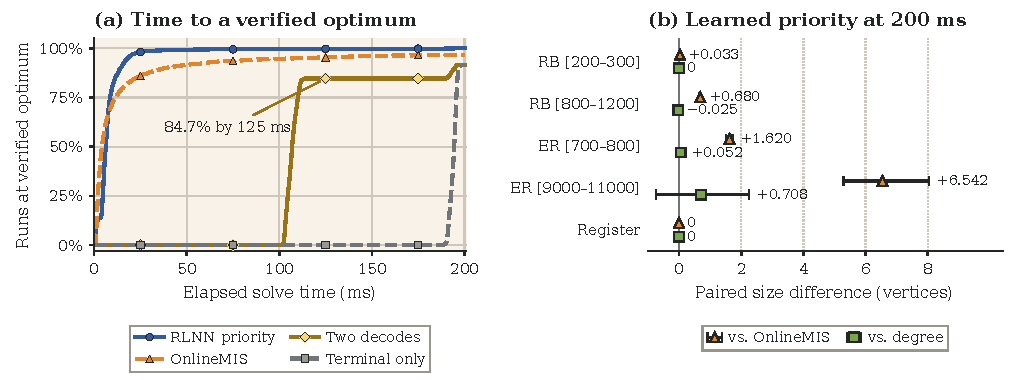
\includegraphics[width=1.0\textwidth]{figures/intro_evidence.pdf}
\caption{\textbf{Delivery timing and the effect of learning.}
(a) Curves show the share of 3,000 small RB graph--seed pairs with an offline-verified optimum already on the host. The particle clock starts at per-graph buffer loading and the resident clock at the host edge list. By 125~ms, two decodes deliver 2,540 optima and terminal-only decoding delivers none. Both reach 2,750 by 200~ms.
(b) Points show learned priority minus each comparator in mean delivered size at 200~ms. Whiskers give pointwise 95\% graph-bootstrap intervals. Small ER uses the single-core interleaved repeat. All three methods tie on every seed of the 14 register graphs. Legend labels: ``RLNN priority'' is the learned ranking of SPRINT-C.}
\label{fig:intro-evidence}
\end{figure*}

